
\section{Sutton1999}

\subsection{BetweenMDPs and semi-MDPs: A framework for temporal abstraction in reinforcement learning}
\begin{frame}{Abstract}{}
  \begin{itemize}
    \item Learning, planning, and representing knowledge at multiple levels of temporal abstraction are key, longstanding challenges for AI
    \item It is considered how these challenges can be addressed within the mathematical framework of reinforcement learning and Markov decision processes (MDPs)
    \item We extend the usual notion of action in this framework to include \textbf{options—closed-loop policies} for taking action over a period of time.
    \item Examples of options include:
    
    \begin{itemize}
        \item picking up an object,
        \item going to lunch, and
        \item traveling to a distant city,
        \item as well as primitive actions ( muscle twitches and joint torques)
    \end{itemize}
    
  \end{itemize}
\end{frame}

\begin{frame}{Abstract}
    \begin{itemize}
        \item In particular, we show that options may be used interchangeably with primitive actions in planning methods such as dynamic programming and in learning methods such as Q-learning.
        \item Formally, a set of options defined over an MDP constitutes a semi-Markov decision process (SMDP), and the theory of SMDPs provides the foundation for the theory of options
        \item However, the most interesting issues concern the interplay between the underlying MDP and the SMDP and are thus beyond SMDP theory.
        \item the results can be obtained without committing to (or ruling out) any particular approach to state abstraction, hierarchy, function approximation, or the macro-utility problem.
    \end{itemize}
\end{frame}

\begin{frame}{Introduction}
    \begin{itemize}
        \item Human decision making routinely involves choice among temporally extended courses of action over a broad range of time scales
        \item {\color{red} This framework has become popular in AI because of its ability to deal naturally with stochastic environments and with the integration of learning and planning [3,4,13,22,64]. Reinforcement learning methods have also proven effective in a number of significant applications [10,42,50,70,77]. MDPs}
        %[10] R.H. Crites, A.G. Barto, Improving elevator performance using reinforcement learning, in: Advances in Neural Information Processing Systems 8,MIT Press, Cambridge, MA, 1996, pp. 1017–1023.
        %[42] P. Marbach, O. Mihatsch, M. Schulte, J.N. Tsitsiklis, Reinforcement learning for call admission control in routing in integrated service networks, in: Advances in Neural Information Processing Systems 10,Morgan Kaufmann, SanMateo, CA, 1998, pp. 922–928.
        %[50] J. Nie, S. Haykin, A Q-learning based dynamic channel assignment technique for mobile communication systems, IEEE Transactions on Vehicular Technology, to appear.
        %[70] S.P. Singh, D. Bertsekas, Reinforcement learning for dynamic channel allocation in cellular telephone systems, in: Advances in Neural Information Processing Systems 9, MIT Press, Cambridge, MA, 1997, pp. 974–980.
        %[77] G.J. Tesauro, Temporal difference learning and TD-Gammon, Comm. ACM 38 (1995) 58–68.
    \end{itemize}
\end{frame}

\begin{frame}{Introduction}
    \begin{itemize}
        \item MDPs as they are conventionally conceived do not involve temporal abstraction or temporally extended action.
        \begin{itemize}
            \item based on a discrete time step: the unitary action taken at time t affects the state and reward at time $t + 1$
            \item there is no notion of a course of action persisting over a variable period of time
            \pause
            \item \textbf{conventional MDP methods are unable to take advantage of the simplicities and efficiencies sometimes available at higher levels of temporal abstraction}
            \item \textbf{\color{red} on the other hand, temporal abstraction can be introduced into reinforcement lerning in a variety of ways [2,8,11,12,14,16,19,26,28, 31,32,38,40,44,45,53,56,57,59,63,68,69,71,73,78–82].}
            %[2] M. Asada, S. Noda, S. Tawaratsumida, K. Hosada, Purposive behavior acquisition for a real robot by vision- based reinforcement learning, Machine Learning 23 (1996) 279–303.
            %[8] L. Chrisman, Reasoning about probabilistic actions at multiple levels of granularity, in: Proc. AAAI Spring Symposium: Decision-Theoretic Planning, Stanford University, 1994.
            %[11] P. Dayan, Improving generalization for temporal difference learning: The successor representation, Neural Computation 5 (1993) 613–624.
            %[12] P. Dayan, G.E. Hinton, Feudal reinforcement learning, in: Advances in Neural Information Processing Systems 5,Morgan Kaufmann, SanMateo, CA, 1993, pp. 271–278.
            %[14] T. Dean, S.-H. Lin, Decomposition techniques for planning in stochastic domains, in: Proc. IJCAI-95, Montreal, Quebec, Morgan Kaufmann, San Mateo, CA, 1995, pp. 1121–1127. See also Technical Report CS-95-10, Brown University, Department of Computer Science, 1995.
            %[16] T.G. Dietterich, The MAXQ method for hierarchical reinforcement learning, in: Machine Learning: Proc. 15th International Conference, Morgan Kaufmann, SanMateo, CA, 1998, pp. 118–126.
            %[19] C. Drummond, Composing functions to speed up reinforcement learning in a changing world, in: Proc. 10th European Conference onMachine Learning, Springer, Berlin, 1998.
            %[26] M. Hauskrecht, N.Meuleau, C. Boutilier, L.P. Kaelbling, T. Dean, Hierarchical solution ofMarkov decision processes using macro-actions, in: Uncertainty in Artificial Intelligence: Proc. 14th Conference, 1998, pp. 220–229.
            %[28] M. Huber, R.A. Grupen, A feedback control structure for on-line learning tasks, Robotics and Autonomous Systems 22 (3–4) (1997) 303–315.
            %[31] L.P. Kaelbling, Hierarchical learning in stochastic domains: Preliminary results, in: Proc. 10th International Conference onMachine Learning, Morgan Kaufmann, SanMateo, CA, 1993, pp. 167–173.
            %[32] Zs. Kalmár, Cs. Szepesvári, A. Lörincz, Module based reinforcement learning: Experiments with a real robot, Machine Learning 31 (1998) 55–85 and Autonomous Robots 5 (1998) 273–295 (special joint issue).
            %[38] L.-J. Lin, Reinforcement learning for robots using neural networks, Ph.D. Thesis, Carnegie Mellon University, Technical Report CMU-CS-93-103, 1993.
            %[40] S.Mahadevan, J. Connell, Automatic programming of behavior-based robots using reinforcement learning, Artificial Intelligence 55 (2–3) (1992) 311–365.
            %[44] A. McGovern, R.S. Sutton, Macro-actions in reinforcement learning: An empirical analysis, Technical Report 98-70, University ofMassachusetts, Department of Computer Science, 1998.
            %[45] N.Meuleau,M. Hauskrecht, K.-E.Kim, L. Peshkin, L.P.Kaelbling, T.Dean, C. Boutilier, Solving very large weakly coupled Markov decision processes, in: Proc. AAAI-98,Madison,WI, 1998, pp. 165–172.
            %[53] R. Parr, S.Russell, Reinforcement learning with hierarchies ofmachines, in:Advances inNeural Information Processing Systems 10,MIT Press, Cambridge, MA, 1998, pp. 1043–1049.
            %[56] D. Precup, R.S. Sutton, S.P. Singh, Planning with closed-loop macro actions, in:Working Notes 1997 AAAI Fall Symposium onModel-directed Autonomous Systems, 1997, pp. 70–76.
            %[57] D. Precup, R.S. Sutton, S.P. Singh, Theoretical results on reinforcement learning with temporally abstract options, in: Proc. 10th European Conference onMachine Learning, Springer, Berlin, 1998.
            %[59] M. Ring, Incremental development of complex behaviors through automatic construction of sensory-motor hierarchies, in: Proc. 8th International Conference on Machine Learning, Morgan Kaufmann, San Mateo, CA, 1991, pp. 343–347.
            %[63] J. Schmidhuber, Neural sequence chunkers, Technische Universität München, TR FKI-148-91, 1991.
            %[68] S.P. Singh, Transfer of learning by composing solutions of elemental sequential tasks, Machine Learning 8 (3/4) (1992) 323–340.
            %[69] S.P. Singh, A.G. Barto, R.A. Grupen, C.I. Connolly, Robust reinforcement learning in motion planning, in: Advances in Neural Information Processing Systems 6,Morgan Kaufmann, SanMateo, CA, 1994, pp. 655– 662.
            %[71] R.S. Sutton, TD models: Modeling the world at a mixture of time scales, in: Proc. 12th International Conference onMachine Learning, Morgan Kaufmann, SanMateo, CA, 1995, pp. 531–539.
            %[73] R.S. Sutton, B. Pinette, The learning of world models by connectionist networks, in: Proc. 7th Annual Conference of the Cognitive Science Society, 1985, pp. 54–64
            %[78] T. Thrun, A. Schwartz, Finding structure in reinforcement learning, in: Advances in Neural Information Processing Systems 7,Morgan Kaufmann, SanMateo, CA, 1995, pp. 385–392.
            %[79] M. Uchibe, M. Asada, K. Hosada, Behavior coordination for a mobile robot using modular reinforcement learning, in: Proc. IEEE/RSJ International Conference on Intelligent Robots and Systems, 1996, pp. 1329– 1336.
            %[80] C.J.C.H.Watkins, Learning with delayed rewards, Ph.D. Thesis, Cambridge University, 1989.
            %[81] M.Wiering, J. Schmidhuber, HQ-learning, Adaptive Behavior 6 (2) (1997) 219–246.
            %[82] L.E. Wixson, Scaling reinforcement learning techniques via modularity, in: Proc. 8th International Conference onMachine Learning, Morgan Kaufmann, SanMateo, CA, 1991, pp. 368–372
        \end{itemize}
    \end{itemize}
\end{frame}

\begin{frame}{Introduction}
    What is the minimal extension of the reinforcement learning framework that allows a general treatment of temporally abstract knowledge and action?
    \pause
    \\
    
    
    Semi-Markov decision processes (SMDPs), as pioneered by Bradtke and Duff [5],  Mahadevan et al. [41], and Parr[52]
    %[5] S.J. Bradtke, M.O. Duff, Reinforcement learning methods for continuous-time Markov decision problems, in: Advances in Neural Information Processing Systems 7,MIT Press, Cambridge,MA, 1995, pp. 393–400.
    %[41] S.Mahadevan, N.Marchalleck, T. Das, A. Gosavi, Self-improving factory simulation using continuous-time average-reward reinforcement learning, in: Proc. 14th International Conference onMachine Learning, 1997, pp. 202–210.
    %[52] R. Parr, Hierarchical control and learning for Markov decision processes, Ph.D. Thesis, University of California at Berkeley, 1998.
\end{frame}

\begin{frame}{Introduction}
    \begin{itemize}
        \item SMDPs are a special kind of MDP appropriate for modeling continuous-time discrete-event systems.
        \begin{itemize}
            \item the actions take variable amounts of time and are intended to model temporally-extended courses of action
            \item the existing theory of SMDPs specifies how to model the results of these actions and how to plan with them
            \item exisitng SMDP work is limited beacuse the temporally extended actions are treated as indivisible and unknown units
            \item there is no attempt in SMDP theory tolook inside the temporally extended actions, to examine or modify their strucutre in terms of lower-level actions: \textbf{this is the essence of analyzing temporally abstract actions}
        \end{itemize}
        \item Goal directed behavior involves multiple overlapping scales at which decisions are made and modified
    \end{itemize}
\end{frame}

\begin{frame}{Introduction}
    \begin{itemize}
        \item SMDP actions (the options) are no longer black boxes,  but policies in the base MDP which can be examined, changed, learned, and planned in their own right
        \begin{itemize}
            \item The underlying base system is an MDP, with regular, single-step transitions, while the options define potentially larger transitions, like those of an SMDP, that may last for a number of discrete steps
            %\item Base problem it is a conventional discrete-time MDP, but also consider courses of action within the MDP whose results are state transitions of extended and variable duration: \textbf{options}
            \pause
            \item Any fixed set of options defines a discrete-time SMDP embedded within the original MDP
            \begin{figure}
                \centering
                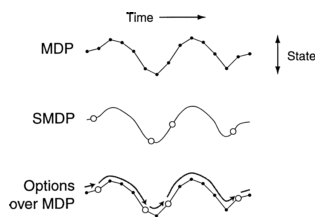
\includegraphics[scale=0.45]{img/options.png}
                %\caption{State trajectory}
                \label{fig:options}
            \end{figure}
        \end{itemize}
    \end{itemize}
\end{frame}

\begin{frame}{MDP Framework}
    \begin{itemize}
        \item Framework of dicrete-time, finite Markov decision process (MDP)
        \begin{itemize}
            \item basis for our extension to temporally extended courses of action
            \item learning agent interacts with an environment (lowest-level time scale, t= 0, 1, 2, ...)
            \item on each time step, t, the agent perceives the state of the environment, $s_t \in S$, and on that basis chooses a primitive action, $a_t \in A_{s_t}$
            \item in response to each action $a_t$, the environment produces one step later a numerical reward $r_{t+1}$ and a next state $s_{t+1}$
            \item If $S$ and $A$ are finite then the environment's transition dynamics can be modeled by one-step state-transition probabilities and one-step expected rewards.
            \begin{itemize}
                \item $p^a_{ss'} = Pr\{s_{t+1}=s'|s_t=s, a_t=a\}$
                \item $r^a_s = E\{r_{t+1}|s_t=s, a_t=a\}$
            \end{itemize}
        \end{itemize}
    \end{itemize}
\end{frame}

\begin{frame}{MDP Framework}
    \begin{itemize}
        \item Framework of dicrete-time, finite Markov decision process (MDP)
        \begin{itemize}
            \item the agent's objective is to learn a \textbf{Markov policy}, a mapping from states to probabilities of taking each available primitive action, $\pi : S \times A \rightarrow [0,1]$, that maximizes the expected discounted future reward from each state s:
            \item value of state $\rightarrow V^\pi(s)$
            \item $= E\{r_{t+1} + \gamma r_{t+2} + \gamma^2 r_{t+3} + \cdots | s_t = s,\pi\}$
            \item $ = E\{r_{t+1} + \gamma V^\pi(s_t+1)|s_t=s,\pi\}$
            \item $= \sum_{a \in A_s} \pi (s,a) \left [ r^a_s + \gamma \sum_{s'}p^a_{ss'}V^\pi(s') \right ]$
            \item $\pi(s,a)$ is the probability with which the policy $\pi$ chooses action $a \in A_s$ in state $s$, and $\gamma \in [0,1]$ is a \textit{discount-rate} parameter
        \end{itemize}
    \end{itemize}
\end{frame}

\begin{frame}{MDP Framework}
    \begin{itemize}
        \item Framework of dicrete-time, finite Markov decision process (MDP)
        \begin{itemize}
            \item the optimal state-value function\end{itemize}
    \end{itemize}
\end{frame}

\begin{frame}{MDP Framework}
    \begin{itemize}
        \item Framework of dicrete-time, finite Markov decision process (MDP)
        \begin{itemize}
            \item action-value function for policy $\pi \rightarrow Q^\pi (s,a)$\end{itemize}
    \end{itemize}
\end{frame}

\begin{frame}{MDP Framework}
    \begin{itemize}
        \item Framework of dicrete-time, finite Markov decision process (MDP)
        \begin{itemize}
            \item optimal action-value function $Q^* (s,a)$\end{itemize}
    \end{itemize}
\end{frame}

\begin{frame}{MDP Framework}
    \begin{itemize}
        \item Framework of dicrete-time, finite Markov decision process (MDP)
        \begin{itemize}
            \item finally, many tasks are episodic in nature, involving repeated trials, or \textit{episodes}, each ending with a reset to a standard state or state distribution
            \item episodic tasks include a special terminal state (arriving in this state terminates the current episode)
            \item the set of regular states plus the terminal state (if there is one) is denoted $S^+$
            \item thus $s'$ in $p^a_{ss'}$ in general ranges over the set $S^+$ rather than just S as stated earlier
            \item In an episodic task, values are defined by the expected cumulative reward up until termination rather then over the infinite future (or, equivalently, we can consider the terminal state to transition to itself forever with a reward of zero)
            %For more details and background on reinforcement learning see [72]
        \end{itemize}
    \end{itemize}
\end{frame}

\begin{frame}{Options}
    \begin{itemize}
        \item a Markov option executes as follows
        \begin{itemize}
            \item next action $a_t$ is selected according to probability distribution $\pi(s_t,\cdot)$
            \item the environment then makes a transition to state $s_{t+1}$, where the option either terminates, with probability $\beta(s_{t+1})$, or else continues, determining $a_{t+1}$ according to $\pi(s{t+1},\cdot)$, possibly terminating in $s_{t+2}$ according to $\beta(s_{t+2})$
            \begin{itemize}
                \item an option open-the-door might consist of a policy for reaching, grasping and turning the door knob
                \item termination condition for recognizing that the door has been opened, and
                \item an initiation set restricting consideration of open-the-door to states in which a door is present
                \item in episodic tasks, termination of an episode also terminates the current option: maps the terminal state to 1 in all options.
            \end{itemize}
        \end{itemize}
    \end{itemize}
\end{frame}

\begin{frame}{Options}
    \begin{itemize}
        \item The initiation set and termination condition of an option together restrict its range of application in a potentially useful way.
        \begin{itemize}
            \item they limit the range over which the option’s policy needs to be defined. For example:
            a handcrafted policy $\pi$ for a mobile robot to dock with its battery charger might be defined only for states I in which the battery charger is within sight.
            \item The termination condition $\beta$ could be defined to be 1 outside of I and when the robot is successfully docked.
            \item A subpolicy for servoing a robot arm to a particular joint configuration could similarly have a set of allowed starting states, a controller to be applied to them, and a termination condition indicating that either the target configuration has been reached within some tolerance or that some unexpected event has taken the subpolicy outside its domain of application.
            \item For Markov options it is natural to assume that all states where an option might continue are also states where the option might be taken
            % (i.e., that {s: β(s)<1}⊆I). In this case, π need only be defined over I rather than over all of S.
        \end{itemize}
    \end{itemize}
\end{frame}

\begin{frame}{Options}
    \begin{itemize}
        \item Sometimes it is useful for options to “timeout”, to terminate after some period of time has elapsed even if they have failed to reach any particular state.
        \item This is not possible with Markov options because their termination decisions are made solely on the basis of the current state, not on how long the option has been executing.
        \item To handle this and other cases of interest we allow semi-Markov options, in which policies and termination conditions may make their choices dependent on all prior events since the option was initiated.
        \item The decisions of a Markov option may depend only on $s_\tau$, whereas the decisions of a semi-Markov option may depend on the entire preceding sequence $s_t, a_t, r_{t+1}, s_{t+1}, a_{t+1},\cdots,r_\tau, s_\tau$, but not on events prior to $s_t$ (or after $s_\tau$)
        \item \textit{history}: sequence from t to $\tau$ and denote it by $h_{t\tau}$
        \item $\Omega$: set of all histories
    \end{itemize}
\end{frame}

\begin{frame}{Options}
    \begin{itemize}
        \item In semi-Markov options:
        \begin{itemize}
            \item policy and termination condition are functions of possible histories: $\pi:\Omega \times \mathcal{A} \rightarrow [0,1]$ e $\beta:\Omega \rightarrow [0,1]$
            \item also arise if options use a more setailed state representation than available to the policy that selects the options, as in \textit{hierarchical abstract machines} and MAXQ
            \item Finally, note that hierarchical structures, such as options that select other options, can also give rise to higher-level options that are semi-Markov (even if all the lower-level options are Markov). \item Semi-Markov options include a very general range of possibilities.
            %%%[16] T.G. Dietterich, The MAXQ method for hierarchical reinforcement learning, in: Machine Learning: Proc. 15th International Conference, Morgan Kaufmann, SanMateo, CA, 1998, pp. 118–126.
            %%%[52] R. Parr, Hierarchical control and learning for Markov decision processes, Ph.D. Thesis, University of California at Berkeley, 1998
            %%%[53] R. Parr, S.Russell, Reinforcement learning with hierarchies ofmachines, in:Advances inNeural Information Processing Systems 10,MIT Press, Cambridge, MA, 1998, pp. 1043–1049.
        \end{itemize}
    \end{itemize}
\end{frame}

\begin{frame}{Options}
    \begin{itemize}
        \item $\mathcal{O}_s$ are much like the sets of available actions, $\mathcal{A}_s$
        \item Each action $a$ corresponds to an option that is available whenever $a$ is available $(\mathcal{I} = \left \{s: a \in \mathcal{A}_s \right \} )$, that always lasts exactly one step $(\beta(s) = 1, \forall_s \in \matcal{S})$, and that selects $a$ everywhere $(\pi(s,a) = 1, \forall_s \in \mathcal{I})$
        \item The former we refer to as \textit{single-step} or \textit{primitive} options and the latter as \textit{multi-step} options.
        \item $\mathcal{O} = \bigcup_{s \in \mathcal{S}} \mathcal{O}_s$: available options across states
    \end{itemize}
\end{frame}

\begin{frame}{Options}
    \begin{itemize}
        \item Policies over options
        \begin{itemize}
            \item when initiated in a state $s_t$, the Markov policy over options $\mi: \mathcal{S} \times \mathcal{O} \rightarrow [0,1]$ selects an options $o \in \mathcal{O}_s_t$ according to probability distribution $\mi(s_t,\cdot)$
        \end{itemize}
    \end{itemize}
\end{frame}

\begin{frame}{Planning with options - SMDP planning}
    \begin{figure}
        \centering
        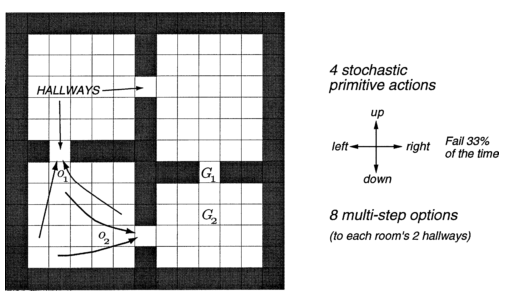
\includegraphics[width=0.6\textwidth]{img/planningOptions.png}
        %\caption{}
        \label{figPlanningOptions}
    \end{figure}
    \begin{itemize}
        \item Action Probability:
        \begin{itemize}
            \item 2/3: the actions cause the agent to move one cell in the corresponding direction; and
            \item 1/3: the agent moves instead in one of the other three directions - each with probability 1/9
        \end{itemize}
        \item if the agent goes to wall then stays in the same cell
        \item consider rewards are zero on all state transitions
    \end{itemize}
\end{frame}

\begin{frame}{Planning with options - SMDP planning}
    \begin{itemize}
        \item In each of the four rooms we provide two built-in hallway options designed to take the agent from anywhere within the room to one of the two hallway cells leading out of the room.
        \item the policy for one hallway option is shown in
        \item The termination condition $beta(s)$ for each hallway option is:
        \begin{itemize}
            \item 0 for states s within the room and
            \item 1 for states outside the room, including the hallway states.
        \end{itemize}
        \item The initiation set \mathcal{I} comprises the states within the roomplus the non-target hallway state leading
        \item Formally, the goal state is a state fromwhich all actions lead to the terminal state with a reward of +1.
        \item $\gamma$ = 0.9
    \end{itemize}
\end{frame}

\begin{frame}{Planning with options - SMDP planning}
    \begin{itemize}
        \item SVI with arious sets of options \mathcal{O}
        \color{red}
        \item $V_k(s) = max \left [ r^o_s + \sum_{s' \in \mathcal{S}}{p_{ss'}^o V_k \hspace{5} 1(s')} \right ]$
        \item $V_0(s) = 0$, except the goal state $V_0(G_1) = 1$
    \end{itemize}
    \begin{figure}
        \centering
        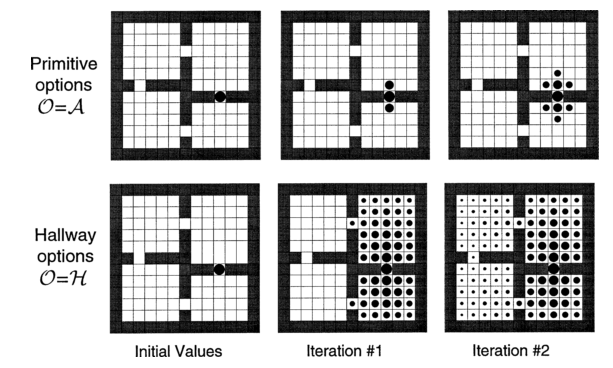
\includegraphics[width=0.5\textwidth]{img/planningOptionsInitG1.png}
        %\caption{Caption}
        \label{figPlanningOptionsInitG1}
    \end{figure}
\end{frame}

\begin{frame}{Planning with options - SMDP planning}
    \begin{figure}
        \centering
        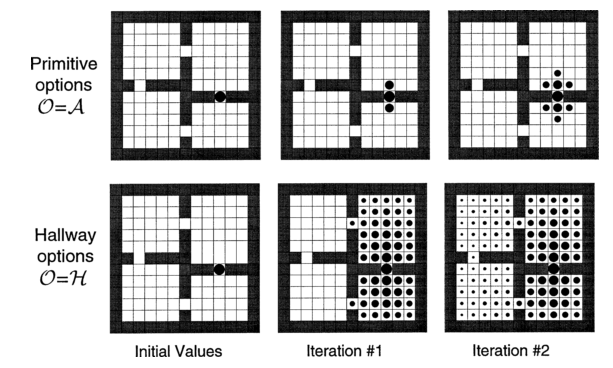
\includegraphics[width=0.5\textwidth]{img/planningOptionsInitG1.png}
        %\caption{Caption}
        \label{figPlanningOptionsInitG1}
    \end{figure}
    \begin{itemize}
        \item The upper part of the figure shows the value function after the first two iterations of SVI using just primitive actions.
        \item In the lower part of the figure are shown the corresponding value functions for SVI with the hallway options.
        \item Rather than planning step-by-step, the hallway options enabled the planning to proceed at a higher level, room-by-room, and thus bemuch faster
    \end{itemize}
\end{frame}

\begin{frame}{Planning with options - SMDP planning}
    \begin{figure}
        \centering
        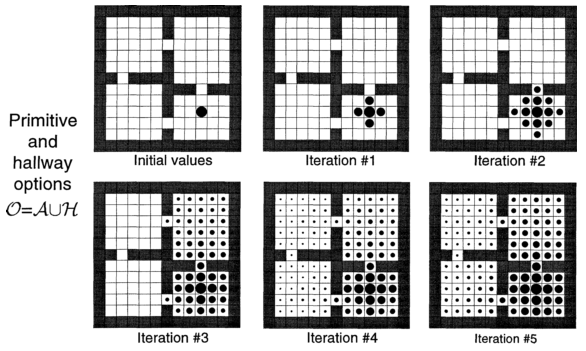
\includegraphics[width=0.5\textwidth]{img/planningOptionsInitG2.png}
        %\caption{Caption}
        \label{figPlanningOptionsInitG1}
    \end{figure}
    \begin{itemize}
        \item Initial progress was due to the models of the primitive options (the actions), but by the third iteration room-to-room planning dominated and greatly accelerated planning.
        \item In large problems, SVI is impractical because the number of states is too large to complete many iterations, often not even one.
    \end{itemize}
\end{frame}

















